\documentclass[11pt]{report}

\usepackage[utf8]{inputenc}
\usepackage{algorithm}
\usepackage{algpseudocode}
\usepackage{hyperref}
\usepackage{graphicx}
\usepackage{subcaption}
\usepackage{booktabs}
\usepackage[square,sort,comma,numbers]{natbib}
\bibliographystyle{abbrv}
\usepackage[font=small,labelfont=bf]{caption}

% Title Page
\title{\textbf{Sports Classification - Temporal vs. Static}}
\author{Object Recognition and Image Understanding \\ \\
  Project Report by \\
  Dominique Cheray and Manuel Krämer}

\begin{document}
\maketitle

\tableofcontents
 
\chapter{Introduction}
\subsubsection{by Manuel Krämer}
Classification is an important task in searching and summarization but most of the previous work doesn't include sports. Therefore, our main goal is to investigate the behaviour of different classfiers on images (static) and videos (temporal) of sport activities. \\
Since neural networks can achieve a very good performance on images we choose
the GoogLeNet \cite{szegedy2015going} and the ResNet \cite{he2016deep}
architecture to train them on single images from the MPII Human Pose Dataset
\cite{andriluka20142d}. To get a better understanding on how the networks work
we implement the CAM algorithm \cite{zhou2016learning} that produces heat maps
where one can see which image regions are considered important by the neural
network to make its prediction. We expect that e.g. the sports equipment is considered as more important by the network than the background. \\
Finally we want to compare this static approach against a dynamic (temporal) approach which includes image sequences of a video. The MPII dataset provides a video for every single frame that is used in the static approach. We need to reduce the feature size in order to get viable data for classification. This is realized by processing the frames through the GoogLeNet until the last hidden layer and concatenating them as described in ch. \ref{TempAnalysis_SVM}. For the final classification a Support Vector Machine is used. We want to achieve an increasing performance for an increasing amount of temporal information (more frames).

\chapter{Fundamentals}
\section{GoogLeNet}
\subsubsection{by Dominique Cheray}
GoogLeNet is a deep convolutional neural network first presented in 2014 and
winner of the ImageNet Large-Scale Visual Recognition Challenge of the same
year. The main building block of this network are the Inception modules which
reduce the number of parameters and at the same time create a deeper and wider
topology. \\
Increasing the size of a deep neural network is the most straightforward way to
improve its performance. This includes increasing the depth of the network, i.e.
the number of levels and the width of the network, i.e. the number of units at
each level. However this approach has two major drawbacks: a bigger size of the
network usually means more parameters, making the network more prone to
overfitting. Furthermore increasing the size of the network also drastically
increases the use of computational resources. To fundamentally solve these
problems, one would have to switch from fully connected to sparsely connected
architectures. However, today's computing infrastructures are very inefficient
when it comes to numerical calculation on non-uniform sparse data structures.
Therefore the main idea of the Inception modules is based on approximating and covering an
optimal local sparse structure in a convolutional network by readily available dense
components \cite{szegedy2015going}. So the authors aim to find the optimal local
construction and to repeat it spatially. \\
They argue that an optimal layered network topology can be constructed by analyzing the
correlation statistics of the preceding layers and clustering units with highly
correlated outputs. In lower layers correlations would concentrate in local and
near-local regions and can therefore be covered by 1x1 convolutions.
Additionally, a smaller number of spatially spread-out clusters can be covered
by convolution over larger patches, i.e. 3x3 an 5x5. The final architecture is a
combination of all those layers with their outputs concatenated into a single
vector which is then used as input to the next layer. Additionally an
alternative pooling path is added since pooling operations have been essential
for the success in convolutional networks \cite{szegedy2015going}. To avoid
computational blow up dimension reduction is applied wherever the computational
requirements would increase too much otherwise. Therefore inexpensive 1x1
convolutions are used to compute reductions before the expensive 3x3 and 5x5
convolutions. The 1x1 convolutions also include a ReLU activation making them
dual-purpose. Figure \ref{InceptionModule} shows the structure of an Inception
module. \\
For the final layout of the network several Inception modules are stacked
upon each other. To decimate the resolution of the grid max-pooling layers are
inserted occasionally.For reasons of memory efficiency lower layers are kept in
traditional convolutional fashion end the Inception modules are only used at
higher levels. This stacking allows for tweaking each module without
uncontrolled blow up in computational complexity. The network ends with global
average pooling followed by dropout and a fully connected layer with softmax for the
classification. The network is 27 layers deep and the overall number of layers
used for its construction is about 100.
\begin{figure}
  \centering
  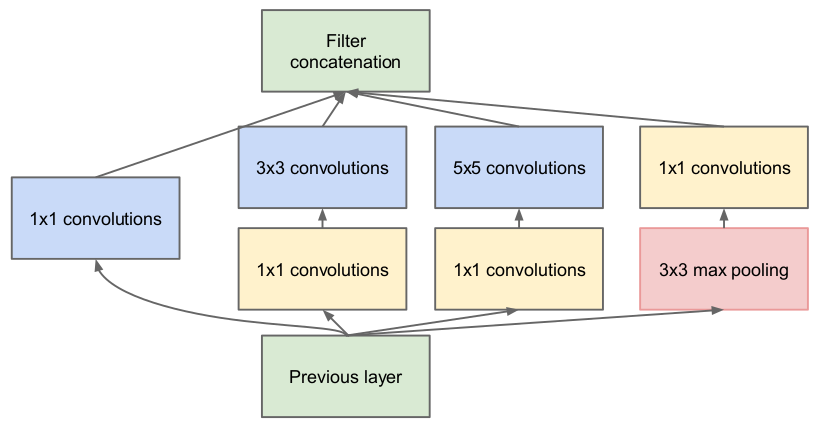
\includegraphics[width=0.5\textwidth]{InceptionModule}
  \caption{Inception module with dimension reduction (taken from \cite{szegedy2015going}).}
  \label{InceptionModule}
\end{figure}

\section{ResNet}
\subsubsection{by Dominique Cheray}
Residual Networks were first presented in 2015 and winner of the ImageNet
Large-Scale Visual Recognition Challenge of the same year. The core idea of
ResNet is the introduction of so-called identity shortcut connections that skip
one or more layers, as shown in figure \ref{ResidualBlock}. A residual block has
two options: either perform a set of functions on the input or skip this step
altogether. \\
The depth of a neural network is of crucial importance for its performance.
However, increasing network depth does not work by simply
stacking layers together. With increasing network depth the accuracy gets saturated
and eventually degrades rapidly and therefore adding more layers to a suitably
deep model leads to higher training error \cite{he2016deep}.
The authors of \cite{he2016deep} argue that stacking layers shouldn't degrade the networks
performance, because one could simply stack identity mappings upon the current
network and the resulting architecture would perform the same. This indicates
that the deeper model should not produce a higher training error than its
shallower counterpart. But optimizing deep networks is difficult and current
solvers cannot find the solution. Therefore they propose a deep residual
learning framework. Instead of hoping each few stacked layers directly fit a
desired underlying mapping they explicitly let these layers fit a residual
mapping. The authors hypothesize that letting the stacked layers fit this
residual mapping is easier than letting them directly fit the desired underlying
mapping. \\
Similar to GoogLeNet several of the residual blocks are stacked upon each other
to construct the final network. It ends with a global average pooling layer
followed by fully connected layer with softmax for the classification. 
\begin{figure}
  \centering
  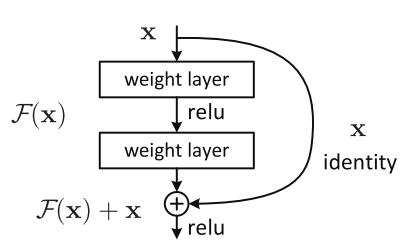
\includegraphics[width=0.4\textwidth]{ResidualBlock}
  \caption{Residual block (taken from \cite{he2016deep}).}
  \label{ResidualBlock}
\end{figure}

\section {Class Activation Mapping}
\label{CAM}
\subsubsection{by Dominique Cheray}
Class Activation Mapping (CAM) is a technique to expose the implicit attention
of Convolutional Neural Networks (CNN) on an image. It highlights the most
informative regions relevant the predicted class \cite{zhou2016learning}. For a
CNN to be used for CAM, its architecture must meet certain requirements. Its
last convolutional layer has to be followed by a layer that performs global
average pooling (GAP) on the convolutional feature maps. The output of the GAP
is then used as features for a fully connected layer that produces the desired
output (categorical or otherwise). \\
The GAP outputs the average of each feature map at the last convolutional layer
and in the fully connected layer a weighted sum of these values is used to
generate the final output. To generate the CAM one now takes the weights of the
fully connected layer belonging to the desired class and the feature maps of the
last convolutional layer and multiplies each feature map by its associated
weight. The weighted feature maps are then added up and upsampled to the size of
the original image. In the resulting image one can identify the image regions
most important to the particular class. Figure \ref{SchematicCAM} shows a
schematic overview of the procedure for generating the class activation maps.
\begin{figure}
  \centering
  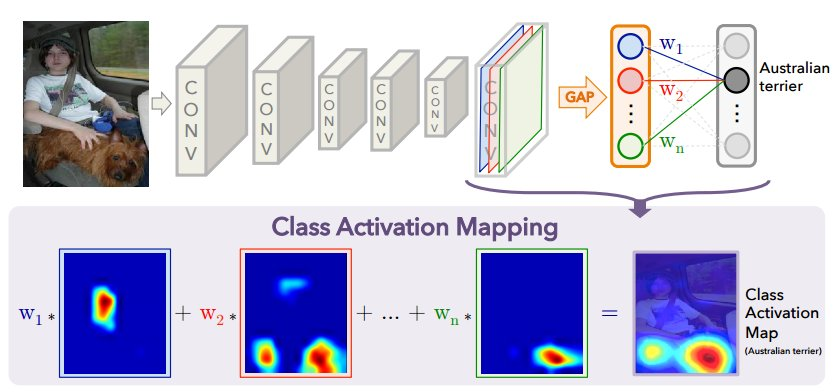
\includegraphics[width=0.9\textwidth]{CAM_graphik}
  \caption{Schematic overview of the procedure for generating the class activation maps (taken from
    \cite{zhou2016learning}).}
  \label{SchematicCAM}
\end{figure}

\section{Data Set}
\label{dataset}
\subsubsection{by Dominique Cheray}
The data set we use in our project is a subset of the MPII Human Pose Dataset
\cite{andriluka20142d}. This data set is a state of the art benchmark for
evaluation of articulated human pose estimation. It includes around
25,000 images and covers 410 human activities. The activities cover a wide range
and span from household activities and leisure activities to sports. Each image
of the data set was extracted from a YouTube video and is provided with an
activity label. In addition the preceding and following unannotated frames are
also provided. \\
For the purpose of this project we concentrate on the sports part of the
data set. In order to keep our data set as large as possible and at the same
time the classes balanced, we select the sports that contain the most
pictures and a similar number of pictures. The remaining data set consists of
1576 images distributed over 10 classes. These classes are basketball, horseback
riding, martial arts, paddleball, rock climbing, rope skipping, skateboarding,
softball, tennis, golf. Figure \ref{plotgrid} gives a little insight into the
data set. 
\begin{figure}
  \centering
  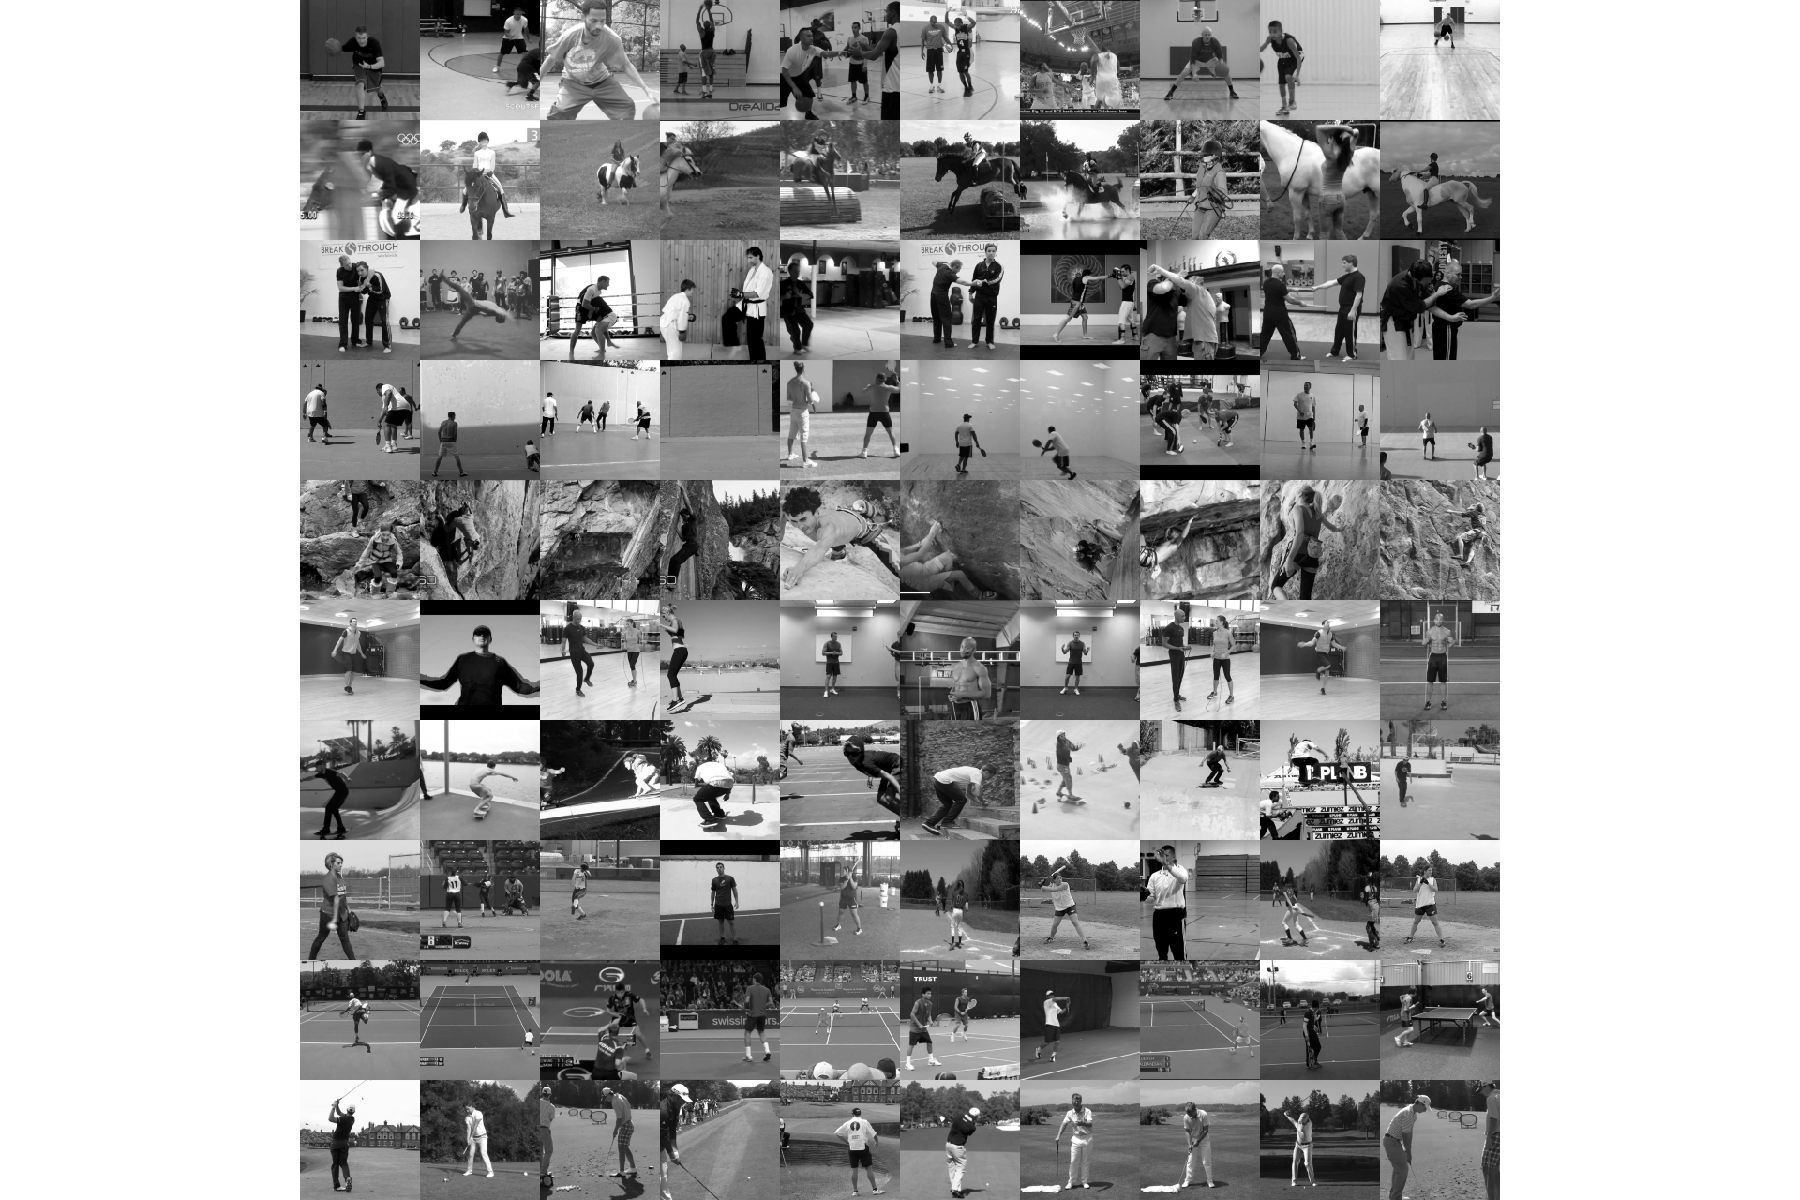
\includegraphics[width=0.6\textwidth]{plotgrid}
  \caption{Samples of the data set - one row is one class.}
  \label{plotgrid}
\end{figure}

\section {Support Vector Machine}
\label{SVM}
\subsubsection{by Manuel Krämer}
The analysis of temporal information can be done by investigating successive frames of a video sequence. We choose, as the method for classification, a Support Vector Machine (SVM) that is suitable because of the comparatively low training effort and a good generalization. \\
In general, the goal of a SVM is to construct a hyperplane in the feature space that separates two classes in a way that maximizes the margin between the two classes. This approach is the reason for the good generalization properties which is better than e.g. the Linear Discriminant Analysis where the margin is not taken into account. The exact behaviour of the margin maximization can be changed with a hyper parameter, often called C-value. This value determines how misclassified points get penalized. If one chooses a high C the model tends to overfitting in order to minimize the training error. A lower C could lead to some mistakes in training but a better generalization, also called soft margin. \\
Since we want to do a multiclass classification the SVM (which is only defined for two classes) uses the so called "one-vs-rest" algorithm. This means that e.g. if you have ten classes you need ten classfiers with class 1 vs all other, class 2 vs all other, etc. These ten classifiers (10 decision surfaces) split the whole feature space into ten separated areas.\\
Another property of the SVM that the kernel-trick ca be used. This means that if you have n-dimensional data the SVM uses a kernel function that computes values in the n+1-dimensional space. This procedure can lead to better results if the data is not linearly separable in n dimension beacuse it maybe is in n+1 dimensions. Often, a radial basis function is used.\\ 
All these aspects make the SVM a good choice for our purpose: It can handle high dimensional data (e.g. images) without a lot of computational effort and it also works well with a small dataset that has only a few instances per class.

\chapter{Methods}
\section{Classification with the Networks}
\subsubsection{by Dominique Cheray}
For the training and testing of the GoogLeNet and the ResNet we randomly
assign 20 \% of the images of each class to the test set and the remaining
images to the training set. Our training set therefore consists of 1266 images
and our test set of 310 images. We train and validate the networks with the
training set and keep the test set for the final testing of the performance
of the networks. \\
Due to the rather small size of our data set we use Data Augmentation to
artificially inflate our data set and avoid overfitting of the networks on the
training data as much as possible. According to the results of \cite{taylor2017improving} we apply
a combination of geometric augmentation and cropping since the authors could
show that applying these two methods improved the performance of CNNs
the most. We therefore first resize the training images to 256x256 pixels and
then apply a random transformation to it (either a flip or a rotation).
Afterwards we extract five 224x224 crops from the transformed image, one crop
out of every corner of the image and one out of the center of the image. Later
during training the prediction of the network is averaged over these five crops
to get one prediction for the underlying original image. \\
We train the networks for 200 epochs using Stochastic Gradient Descent as
optimizer with 0.9 momentum and a start learning rate of 0.01. Every 8 epochs
the learning rate is decreased by 4\%. For the purpose of validating the
training we randomly assign 10\% of the images of the training set to be the validation
set. We then train the parameters of the networks using the remaining training
images and the previously described Data Augmentation methods and validate the
training using the validation set. The test set is left out of the whole
training phase, to prevent overfitting and tuning on it. It is used for the
final evaluation of the predictive accuracy of the networks. \\
To get an idea of which image information the networks use for their
predictions, we implement the Class Activation Mapping described in Chapter
\ref{CAM} and apply it to both networks. Since the architectures of both
networks already 
meet the requirements of the CAM algorithm no changes had to be made to the
networks. For both networks we extract the feature maps of the last
convolutional layer and the weights of the linear layer that follows the GAP
layer. Out of those weights we use the weights that belong to the most
likely class predicted by the networks for a given image. We then multiply each
feature map of the convolutional layer with its associated weight. These
weighted feature maps are then added up and the resulting class activation map
is upsampled to the size of the original image. On this resized class activation
map one can identify the image regions most relevant to the predicted class.  


\section{Temporal Analysis with SVM}
\label{TempAnalysis_SVM}
\subsubsection{by Manuel Krämer}
The approach we used to investigate the temporal information in image sequences (videos) and compare it to a static method like the single frame neural network classification is the following:

\begin{enumerate} 
\item Choose 3,5,7 or 9 successive frames of a video sequence with a spacing of 5 frames (Since the videos aren't that long; if we choose 9 frames we needed to decrease the spacing to 4)
\item Process each single frame through the pretrained GoogLeNet and extract the features from the last hidden layer (which is a feature vector of size 1024)
\item Concatenate all the feature vectors to a single image sequence feature vector
\item Do the classification of these image sequence feature vectors with one of the ten labels (see ch. \ref{dataset}) with a SVM
\end{enumerate}

The described algorithm is shown in fig. \ref{fig_svm}.

\begin{figure}
  \centering
  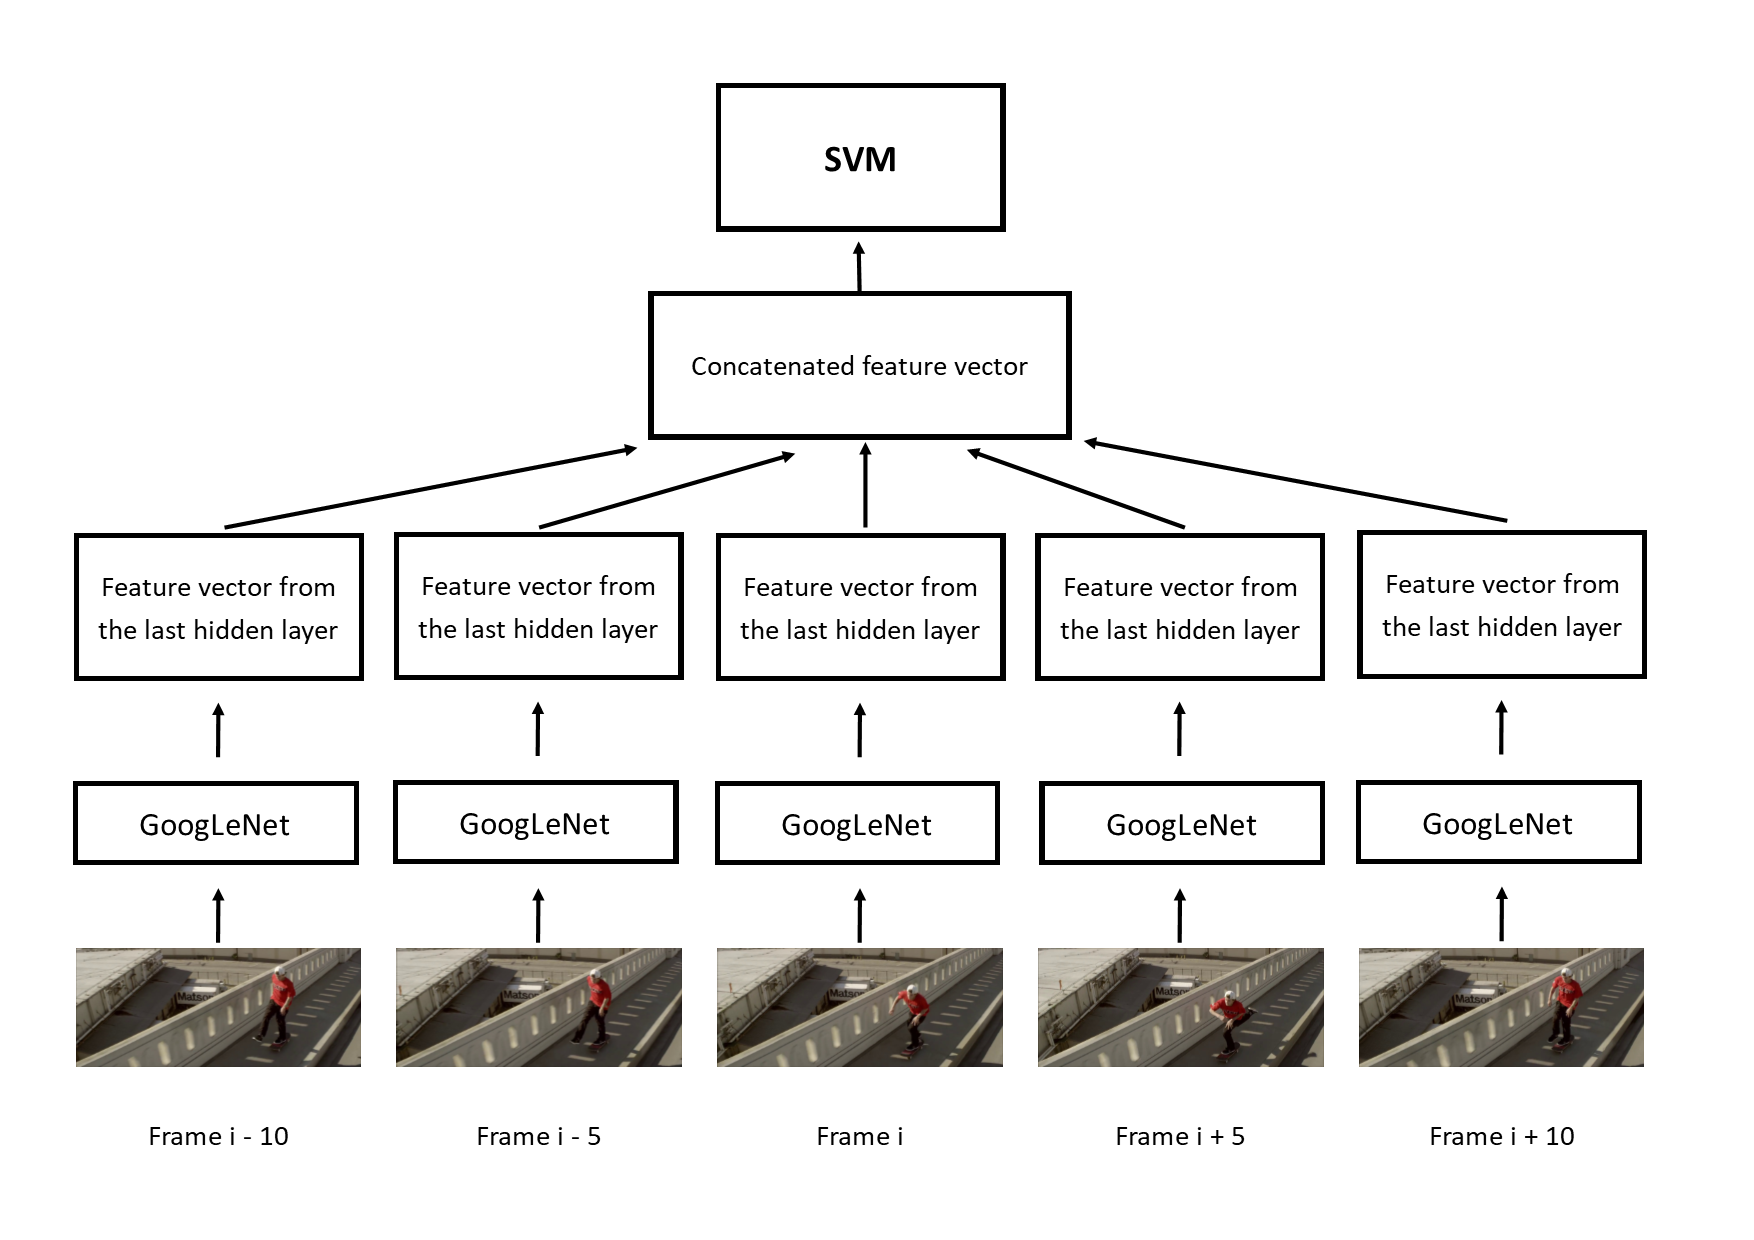
\includegraphics[width=0.7\textwidth]{Illustration_SVM.png}
  \caption{Algorithm of the temporal analysis using a SVM. Here you can see one example of a video sequence of 5 frames}
  \label{fig_svm}
\end{figure}

The Classification with the SVM can be done with several possibilities as you can see in ch. \ref{SVM}. The best results were achieved by a linear SVM (linear kernel), a C-value of 1 and the "one-vs-rest" algorithm. 


\chapter{Results}
\section{Classification with the Networks}
\subsubsection{by Dominique Cheray}

\begin{figure}
  \centering
  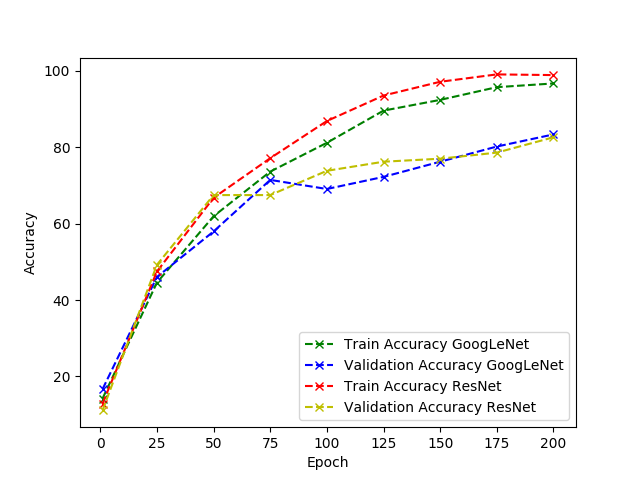
\includegraphics[width=0.7\textwidth]{AccuraciesGraph}
  \caption{Classification Accuracy of GoogLeNet and ResNet for training and
    validation.}
  \label{resultGraphNets}
\end{figure}

\begin{table}[]
  \centering
  \begin{tabular}{|l|l|l|}
    \hline
    & GoogLeNet & ResNet \\ \hline
    Testing Accuracy & 82.3\% & 76.1\% \\ \hline
  \end{tabular}
  \caption{Classification Accuracy of the networks on the test set.}
  \label{resultTableNets}
\end{table}

\begin{figure}
    \centering
    \begin{subfigure}{0.5\textwidth}
        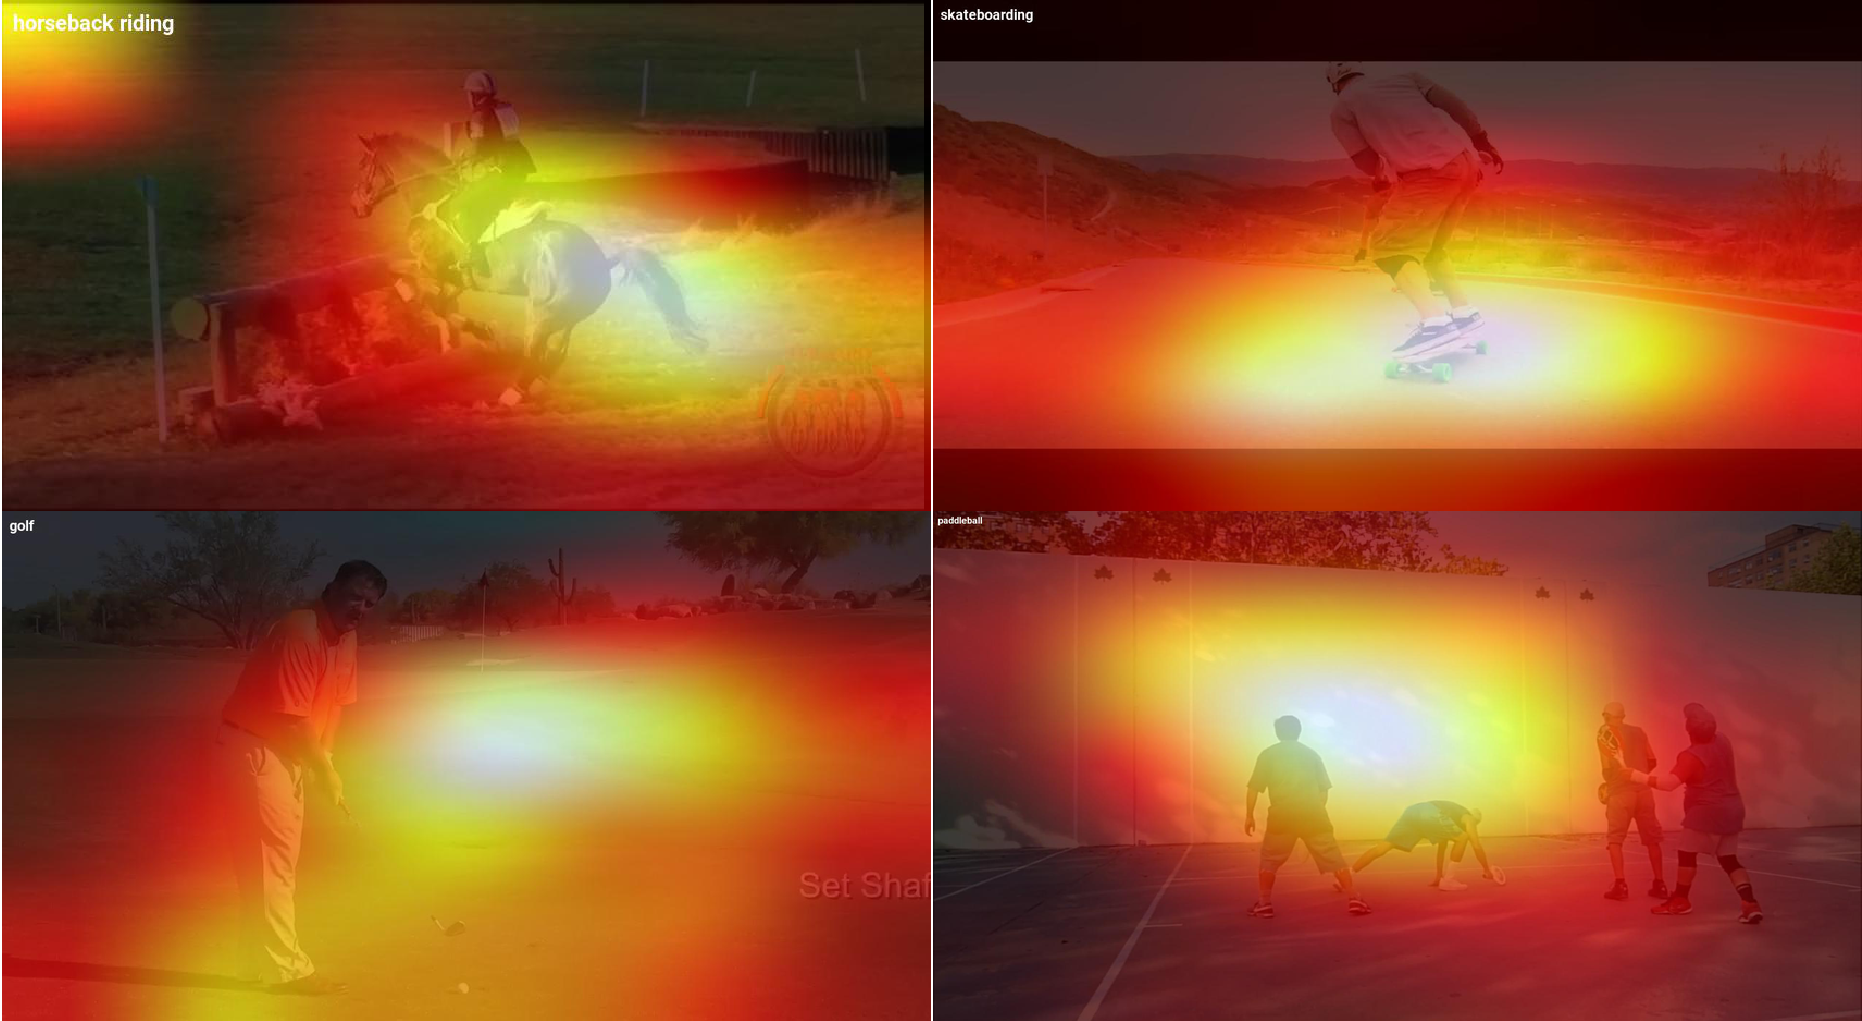
\includegraphics[scale=0.1]{CAMsGoogLeNet}
%        \subcaption{}
%        \label{}
    \end{subfigure}
    \hfill %add desired spacing between images, e. g. ~, \quad, \qquad, \hfill etc. 
      %(or a blank line to force the subfigure onto a new line)
    \begin{subfigure}{0.5\textwidth}
        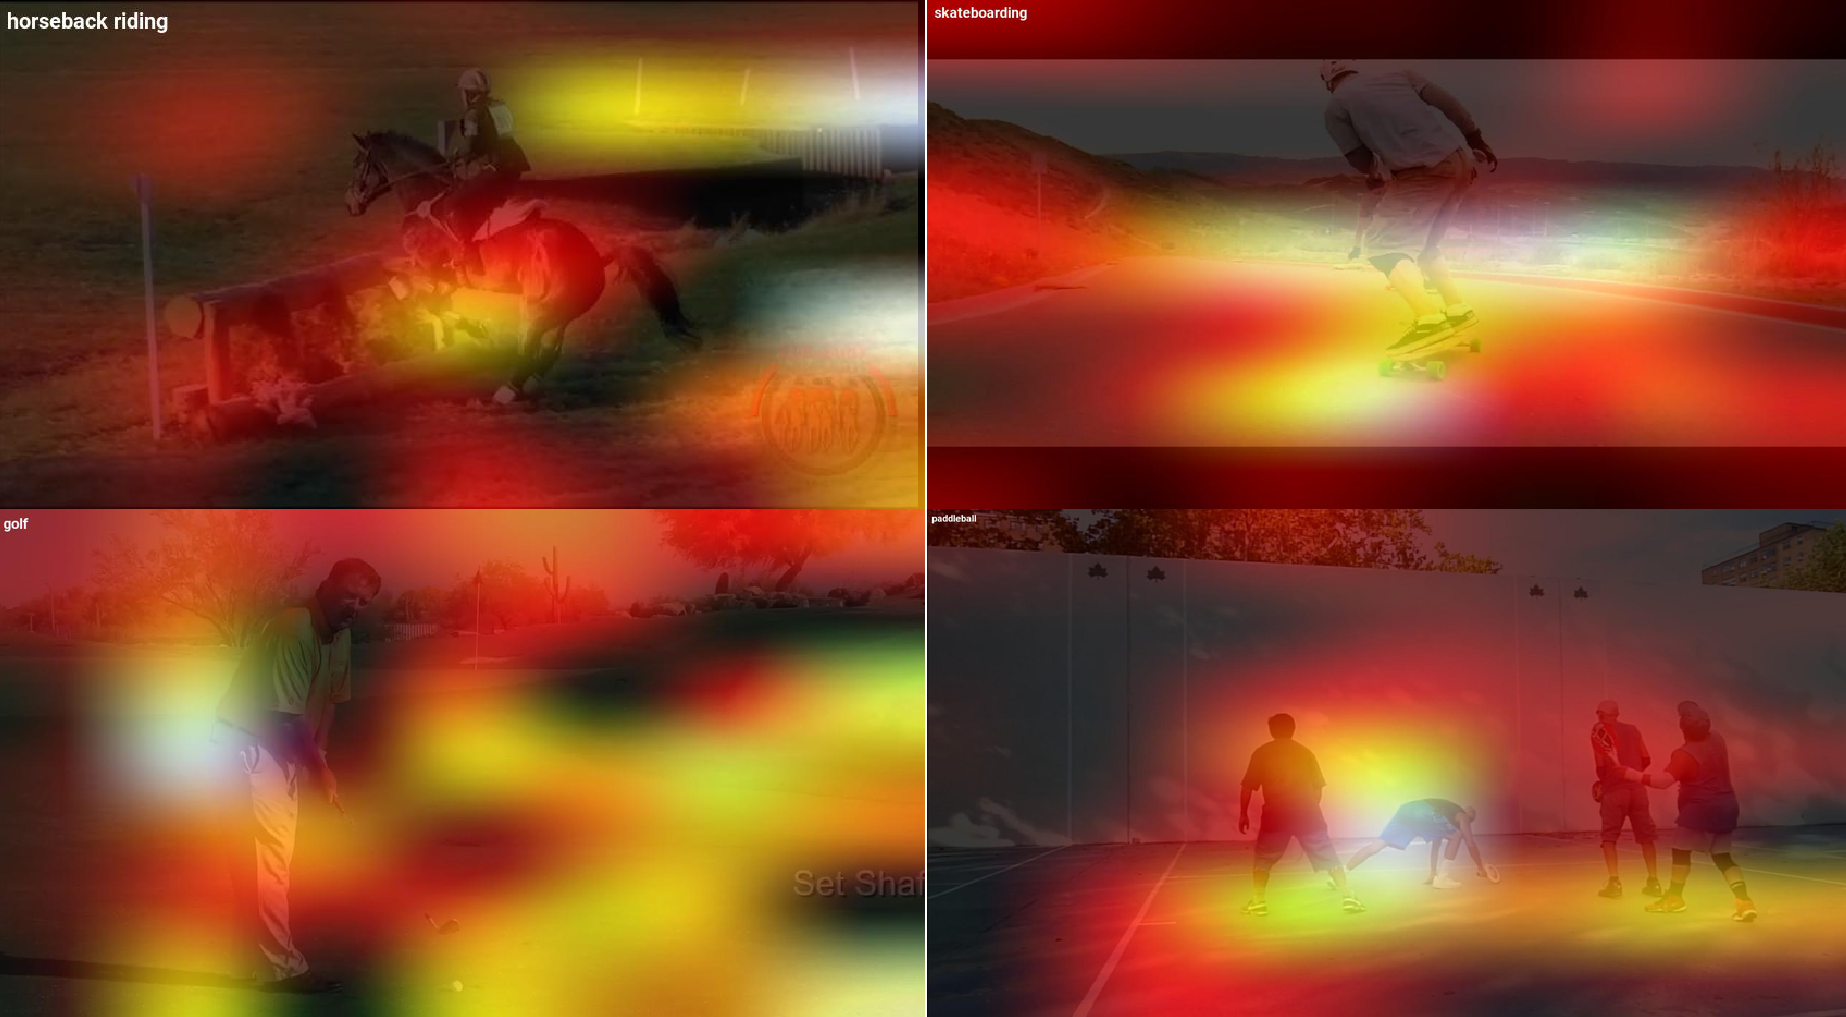
\includegraphics[scale=0.1]{CAMsResNet}
%        \subcaption{}
%        \label{}
      \end{subfigure}
      \caption{Left: Four CAM examples for GoogLeNet. Right: Four CAM examples
        for ResNet}
      \label{CAMImages}
    \end{figure}

Figure \ref{resultGraphNets} shows the classification accuracy of GoogLeNet and
ResNet on the training and validation set during the 200 epochs of training.
For the first 75 or so epochs the training
and validation accuracies of both networks increase about equally fast.
Thereafter the validation accuracies increase much more slowly, sometimes they
even decrease for some epochs and then rise again. Overall both networks perform
very well on the training set and reach accuracies of almost 100\% after the 200
training epochs.
ResNet is even slightly better than GoogLeNet. However on the validation set
both networks only achieve an accuracy of about 80\%. Moreover, on this data
set GoogLeNet is slightly outperforming ResNet. Regarding the test data, the
results look similar to the validation set (see table \ref{resultTableNets}).
With 82.3\% accuracy GoogLeNet is slightly better than ResNet, which only
reaches 76.1\% accuracy. \\
Looking at the class activation mappings that were created for both networks from the images of the
test dataset, it also shows that both networks provide similar results. Figure
\ref{CAMImages} shows four examples of CAMs for both GoogLeNet and ResNet. On
the two top class activation mappings one can see that both networks are more
focused on the horse for the prediction of horseback riding and on the
skateboard for the prediction of skateboarding. For the prediction of golf and
paddleball however, both networks consider the background to be the most
relevant image area to classify the images as shown in the two bottom class
activation mappings for both networks. Overall, the analysis of the CAMs
revealed that for many sports, the networks did not consider the athletes or the
sports equipment as relevant image regions to classify the image. Rather, in
many cases, the background was the most important image information for the two
networks to classify the images. For example when predicting golf as class the
networks mainly looked at the the lawn or when predicting rock climbing they
mainly looked at the surrounding rock face. Only for rope skipping, in almost
all cases, was the athlete the part of the picture the networks focused on.

\section{Temporal Analysis with SVM}
\subsubsection{by Manuel Krämer}
Our results are shown in table \ref{result_table_SMV} and fig. \ref{result_fig_svm}.
One can see that more temporal information (more frames) lead to an increasing accuracy in training. The testing dataset showed the same behaviour besides the fact that at 9 frames it is decreasing compared to 7 frames and the effect is not as significant as one can see for the training.\\
Compared to the static approach, the training accuracy is about the same but the testing accuracy is much worse.

\begin{table}[]
\centering
\begin{tabular}{|l|l|l|}
\hline
3 frames with spacing 5 & 77.6\% & 47.4\% \\ \hline
5 frames with spacing 5 & 88.9\% & 48.4\% \\ \hline
7 frames with spacing 5 & 95.2\% & 52.6\% \\ \hline
9 frames with spacing 4 & 97.3\% & 50.3\% \\ \hline
\end{tabular}
\caption{Classification accuracy of the SVM for 3,5,7 and 9 successive frames of a video sequence}
\label{result_table_SMV}
\end{table}

\begin{figure}
  \centering
  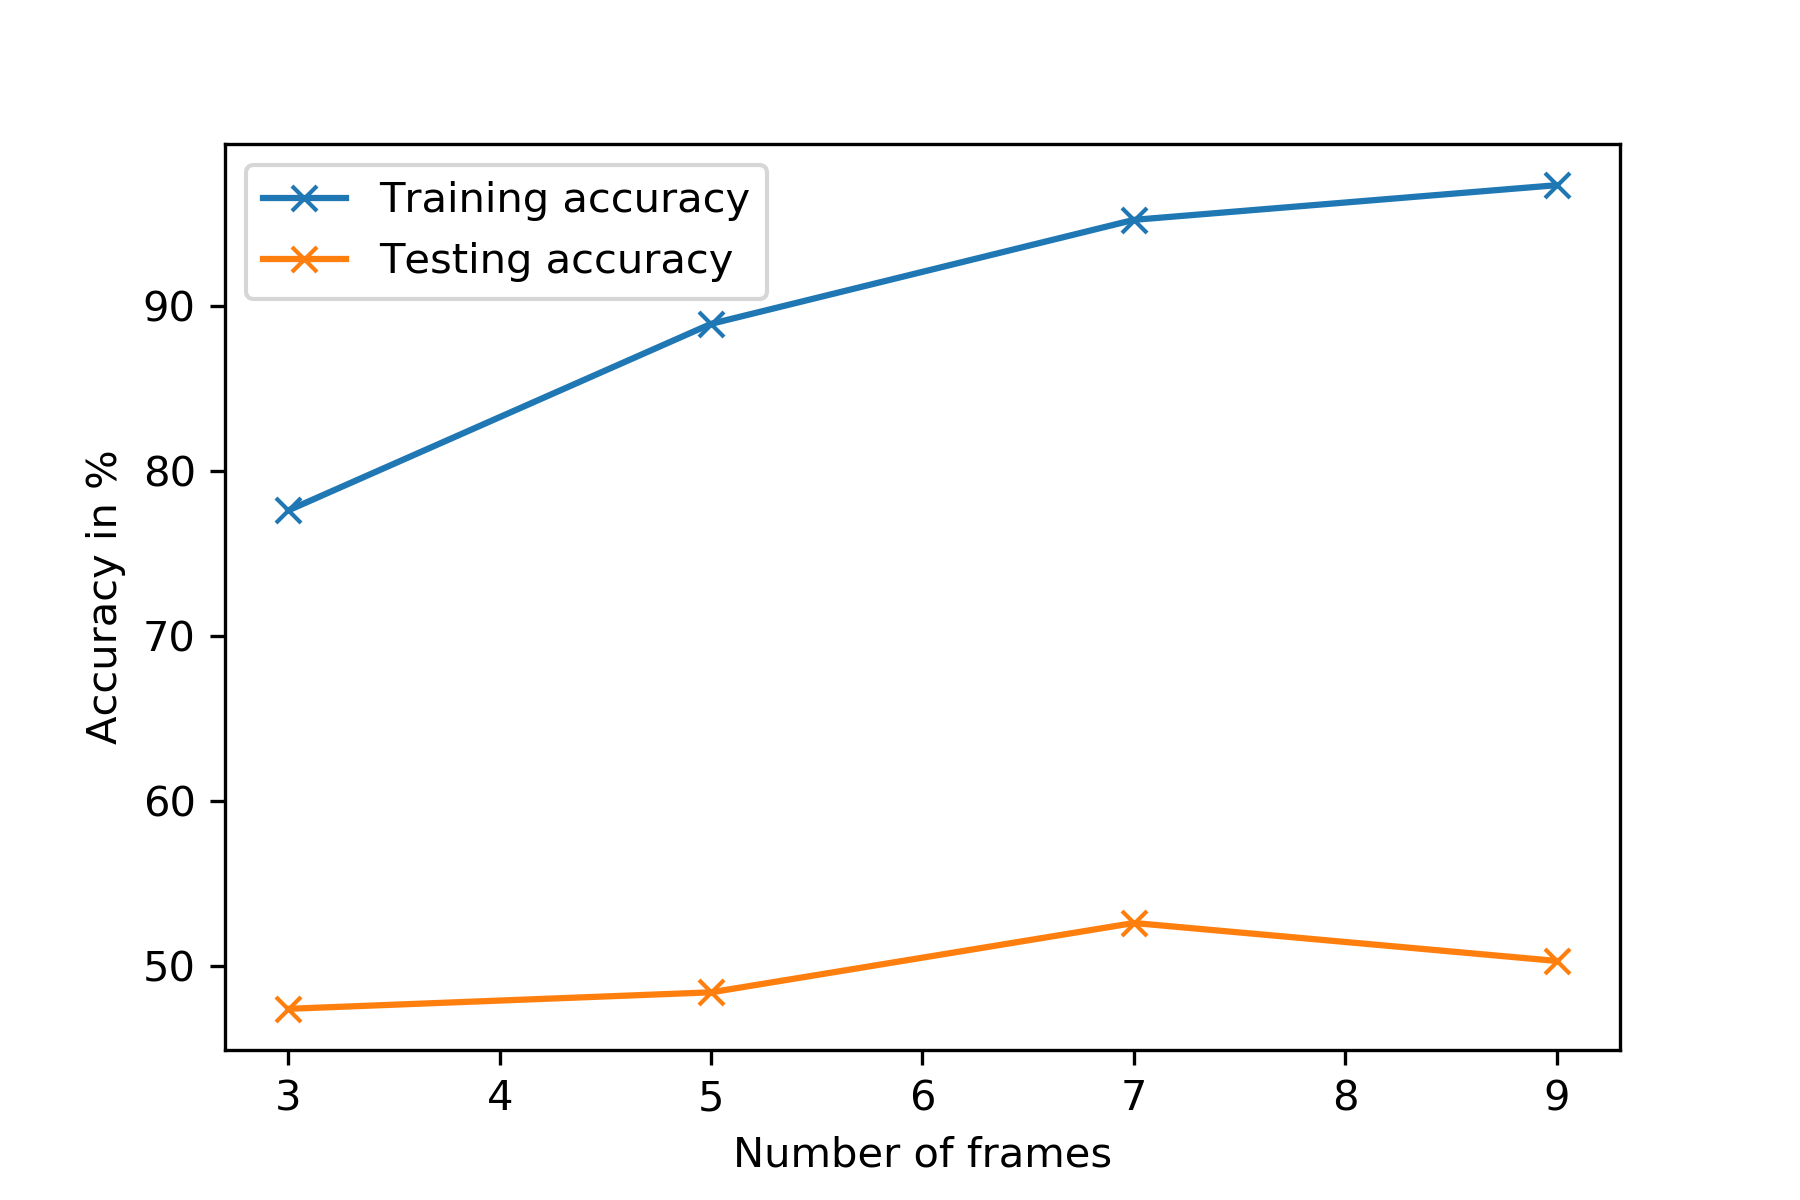
\includegraphics[width=0.7\textwidth]{AccuracySVM.png}
  \caption{Accuracy of the SVM vs. number of images considered for classfication}
  \label{result_fig_svm}
\end{figure}


\chapter{Discussion}
\section{Classification with the Networks}
\subsubsection{by Dominique Cheray}
Considering that our dataset is relatively small and the classes are not fully
balanced, the test accuracy of around 80\% of both networks appears a good
result. However looking at the class activation mappings gives an entirely
different image. Both networks focus mainly on the background to make their
predictions. This is, to a large extent, certainly due to the fact that our
dataset does not involve much variability. For example, if one looks at the
paddleball pictures (see figure \ref{plotgrid} row 4), one can see that they
mostly take place in front of a gray wall, so the background is very similar in
most cases. Or golf for example (see figure \ref{plotgrid} row 10), which always
has a green lawn as background. The networks do not perform well, because they
have, as one might expect, learned to differentiate the sports based on the
sports equipment, but because in many cases the backgrounds of the respective
sports are the same and they have learned to distinguish them and assign them.
The only exception is rope skipping, where the networks are actually mainly
focused on the athlete. These are also the pictures where the backgrounds are
the most different. \\
To address this problem, one could use a larger data set, which has more
variability, especially with regard to the background. However, that might prove
difficult, as most sports always take place against a similar background. Golf
on the lawn, tennis on a tennis court, rock climbing on a rock face et cetera.
Another approach could therefore be to edit the images and remove or unify the
backgrounds before training the neural networks with them. With missing
background or the same background for all sports, the networks can no longer use
this information to differentiate the different sports.

\section{Temporal Analysis with SVM}
\subsubsection{by Manuel Krämer}
The behaviour of the training accuracy one can see in fig. \ref{result_fig_svm} is expected because more frames include more temporal information and this makes the classification more complex but also more accurate. The testing accuracy, indeed is not increasing as much as the training accuracy what means that our model is not generalizing very well. Moreover, there is a decrease from seven to nine frames in the test set due to cuts in some of the videos which leads to the fact that the feature vector contains frames that don't show any relevant information. \\
One reason for the lack of generalization is our dataset which contains many similar frames from one class (e.g. nearly all golf images show green grass and the same distance from the camera to the golfer). Furthermore, the overall testing accuracy is much worse than the one from the static network approach because the SVM and the network are two separated models which means that the extracted features from the GoogLeNet are not optimal for a Support Vector Machine to classify. One solution to this problem would be that we don't use a SVM but another neural network which can be optimized simultaneously with the whole net.
To sum this up, we can verify that more temporal information lead to a better classification performance but we are not able to outperform the neural network. Further work needs to be done in order to study a coupled approach of feature reduction and classification, e.g. a neural net that takes several images and produces a classification with a softmax or a Recurrent Neural Network (RNN) that is often used for video processing.


\bibliography{literature}

\end{document}
